\section{Trusses}

Trusses are support members that are joined together at the ends. The function of a truss is to transmit loads to a support joint. In this section, we will analyze a simplified version of planar trusses called simple trusses, which consist of two-force members connected by frictionless joints/pins.

%starting in lecture 16

%Definition of a truss

\subsection{Truss Assumptions}

The main assumptions for trusses and truss structures are:

\begin{enumerate}
    \item {All loading is applied at the joints.}
    \item{The weight of the truss is negligible.}
\end{enumerate}

Because of these assumptions, all trusses are \textit{two force members}, with the forces on the truss acting along the axis of the member. 
%good summary in lecture 17, slide 5

\subsection{Two Force Member}

A two force member is a rigid body that has two forces (no moments) acting on it in two locations. 

Assumptions of two force members (for equilibrium to hold): 
\begin{enumerate}
\item{$|F_A| = |F_B|$}
\item{$\vec{F_A} + \vec{F_B} = 0$}
\item{$\vec{F_A}$ and $\vec{F_B}$ act along the same line of action.}
\end{enumerate}

\begin{figure*}[!h]
\centering
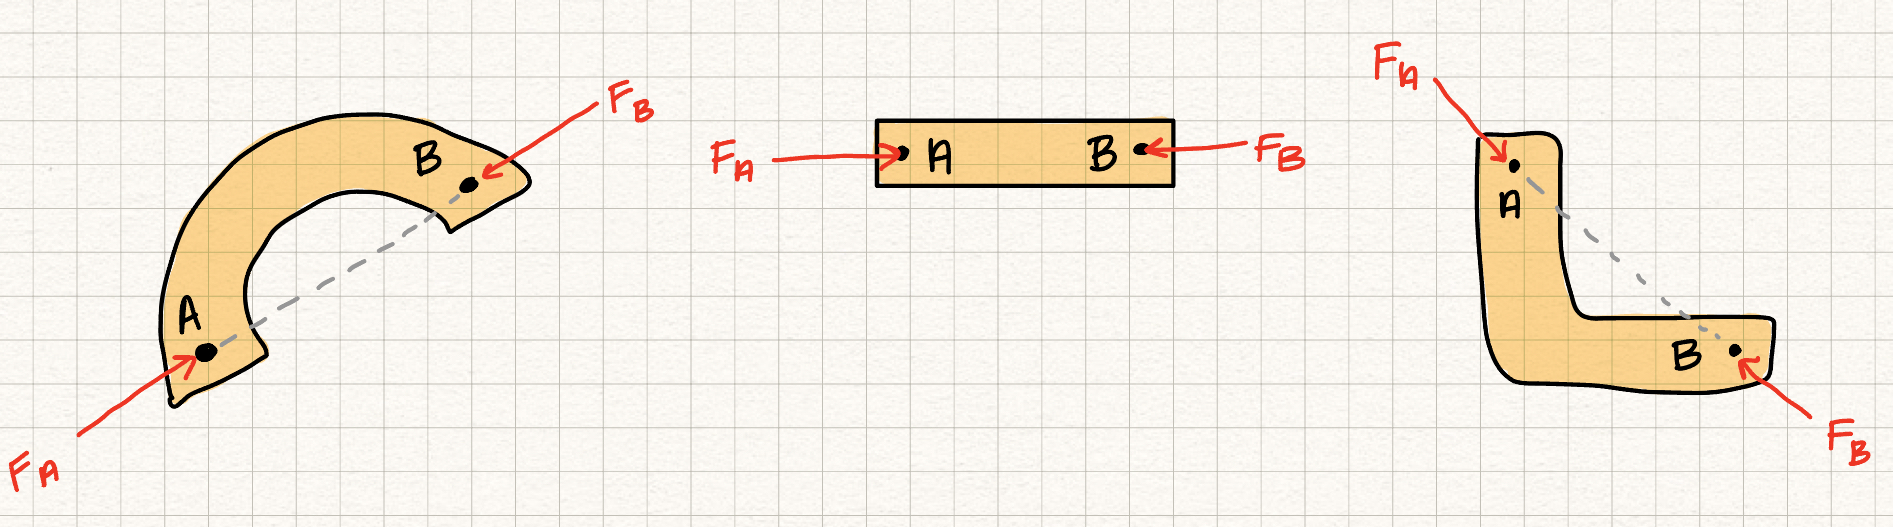
\includegraphics[angle=0, width=5in]{TrussFigures/2ForceMembers.jpg}
\vspace{-2mm}
\caption{\small Examples of different two force members.}
\vspace{-3mm}
\label{Fig:2ForceMembers}
\end{figure*}

    
%Lecture 16
\subsection{Zero Force Member}

Zero force members are members in a truss structure that experience no force. They act as support trusses to add stability, but are not load bearing. There are 2 cases where zero force members occur: 
\begin{enumerate}
    \item Two noncolinear members share a pin with no support or external forces (Zero force member example, left)
    \item Two colinear forces with a third noncolinear force on a pin (zero force member example, right)
\end{enumerate}

\begin{figure*}[!h]
\centering
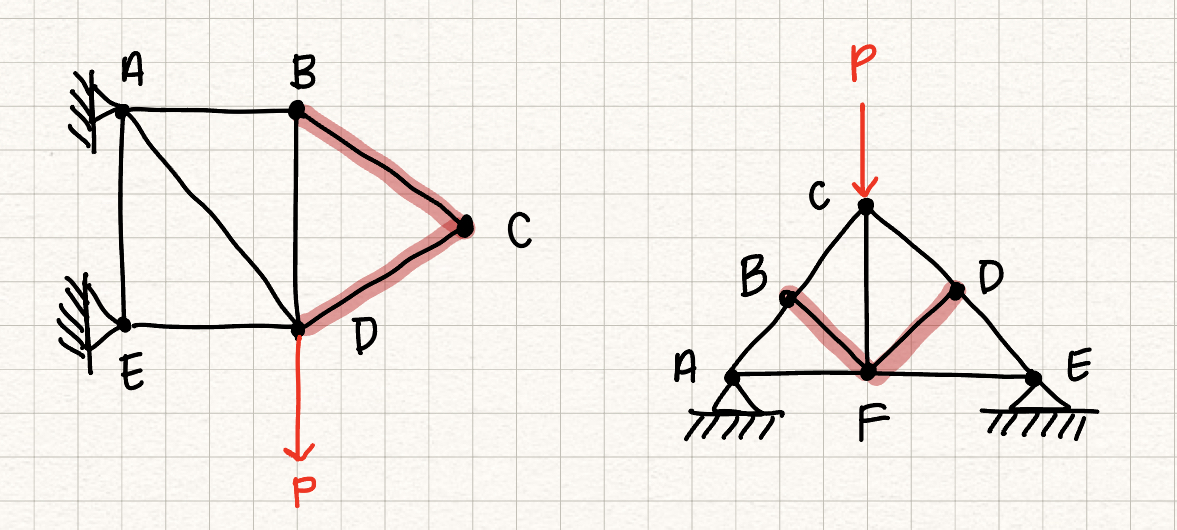
\includegraphics[angle=0, width=5in]{TrussFigures/0ForceMembers.jpg}
\vspace{-2mm}
\caption{\small Examples of different zero force members, highlighted in red.}
\vspace{-3mm}
\label{Fig:0ForceMembers}
\end{figure*}

\blue{Insert content here from TAM 212 reference page - Free Body Diagrams - Rigid Bodies - Trusses section. This has a really good analysis of eliminating zero force members to simplify the structure}

%lecture 18

\subsection{Truss Analysis: Joints}

\begin{figure*}[!h]
\centering
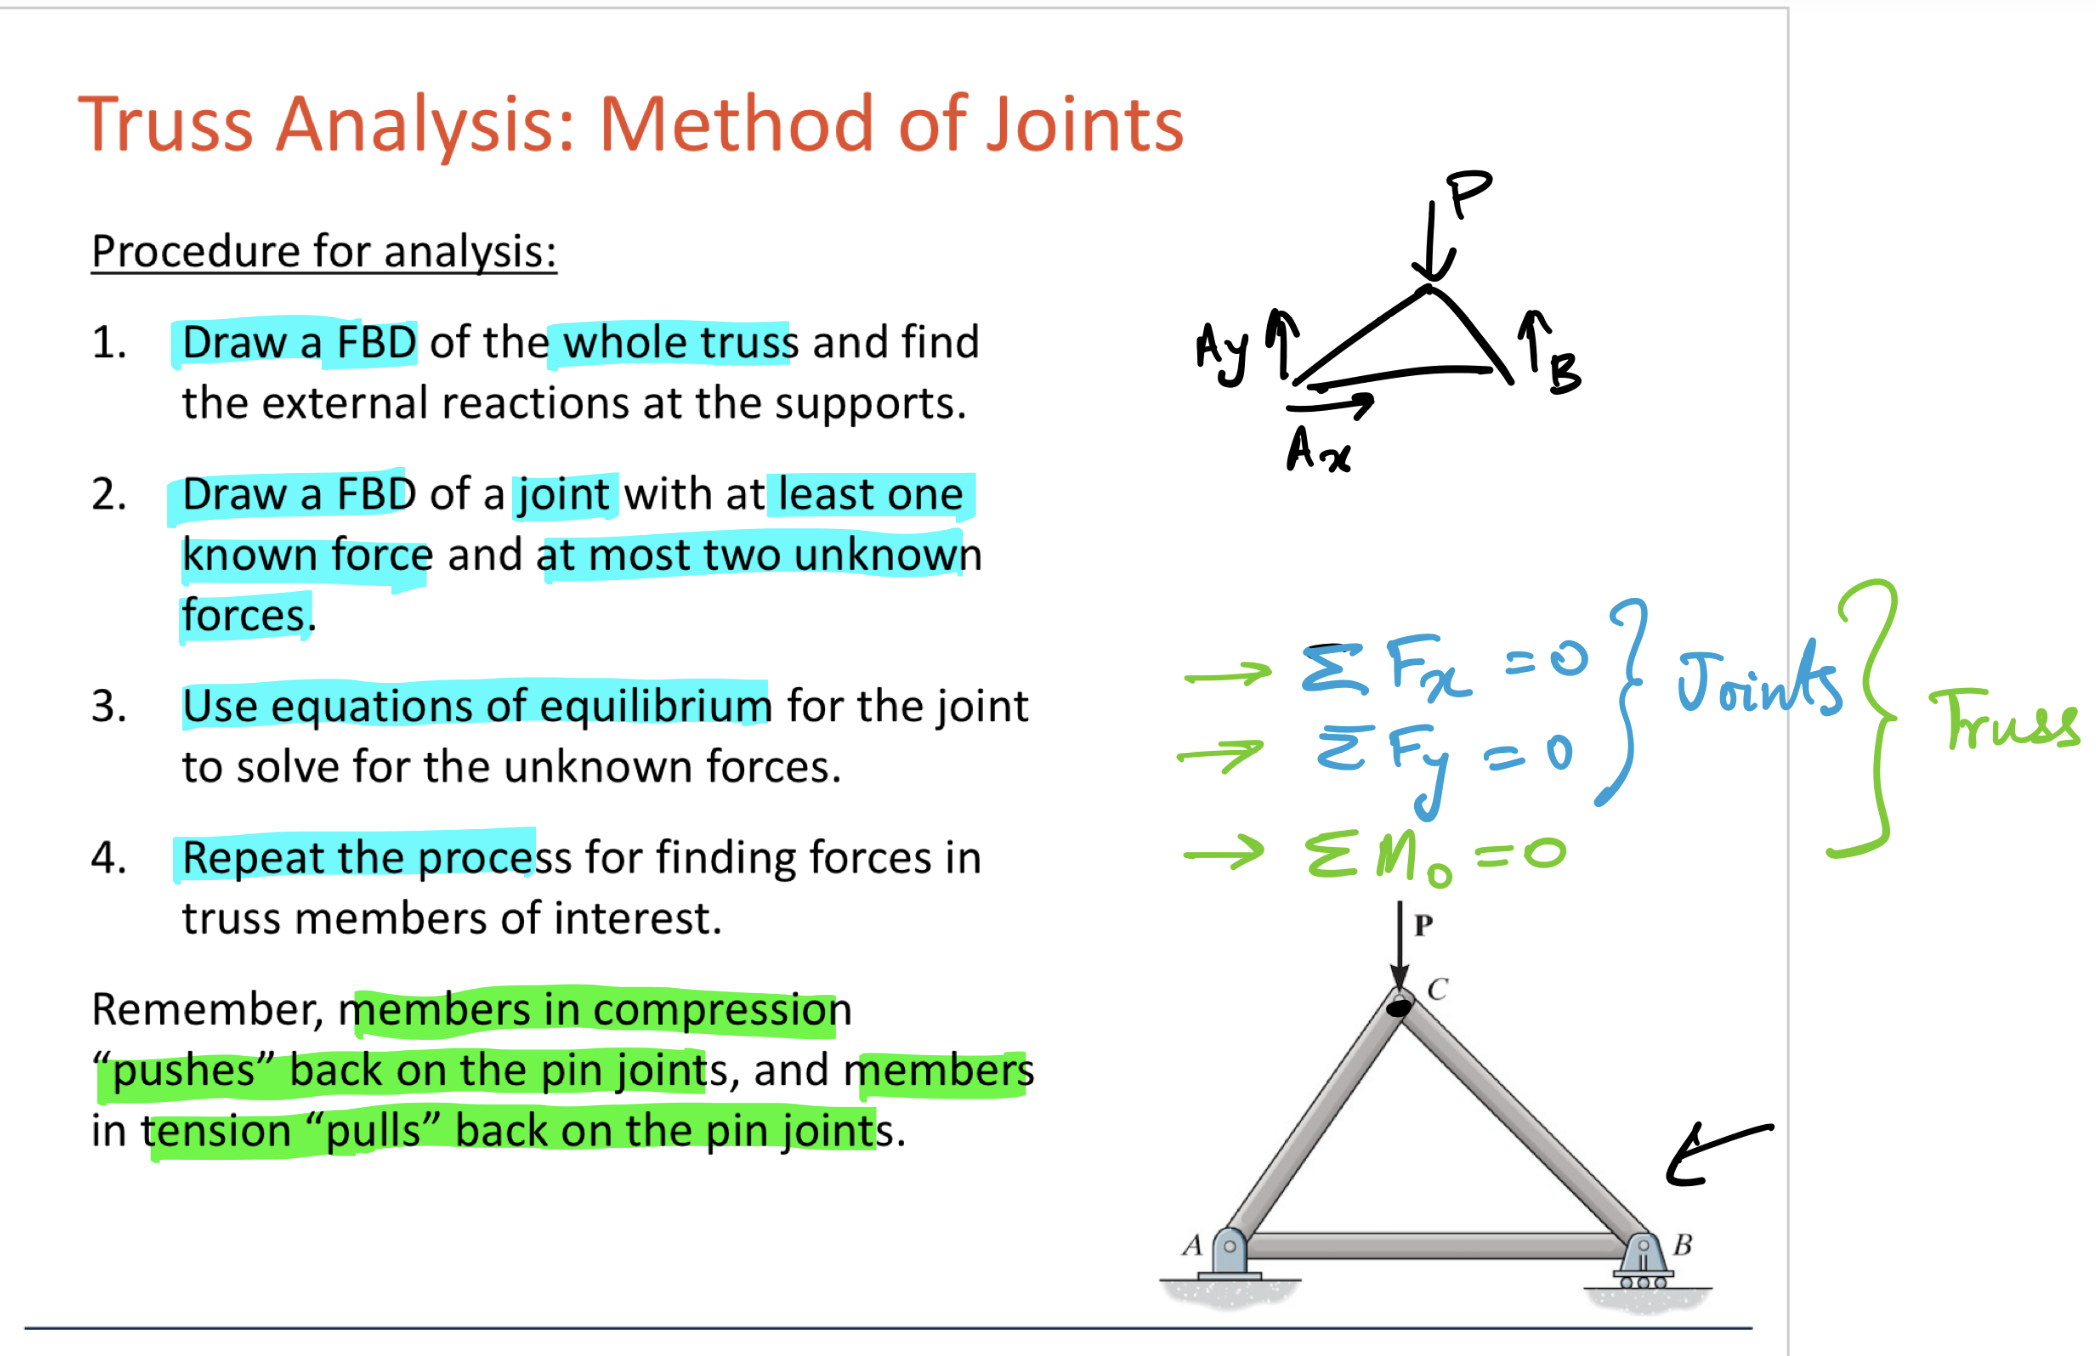
\includegraphics[angle=0, width=5in]{TrussFigures/MethodofJoints.png}
\vspace{-2mm}
\caption{\small \blue{Taken from TAM 210 Lecture 17 notes}}
\vspace{-3mm}
\label{Fig:MethodofJoints}
\end{figure*}

\subsection{Truss Analysis: Sections}

\begin{figure*}[!h]
\centering
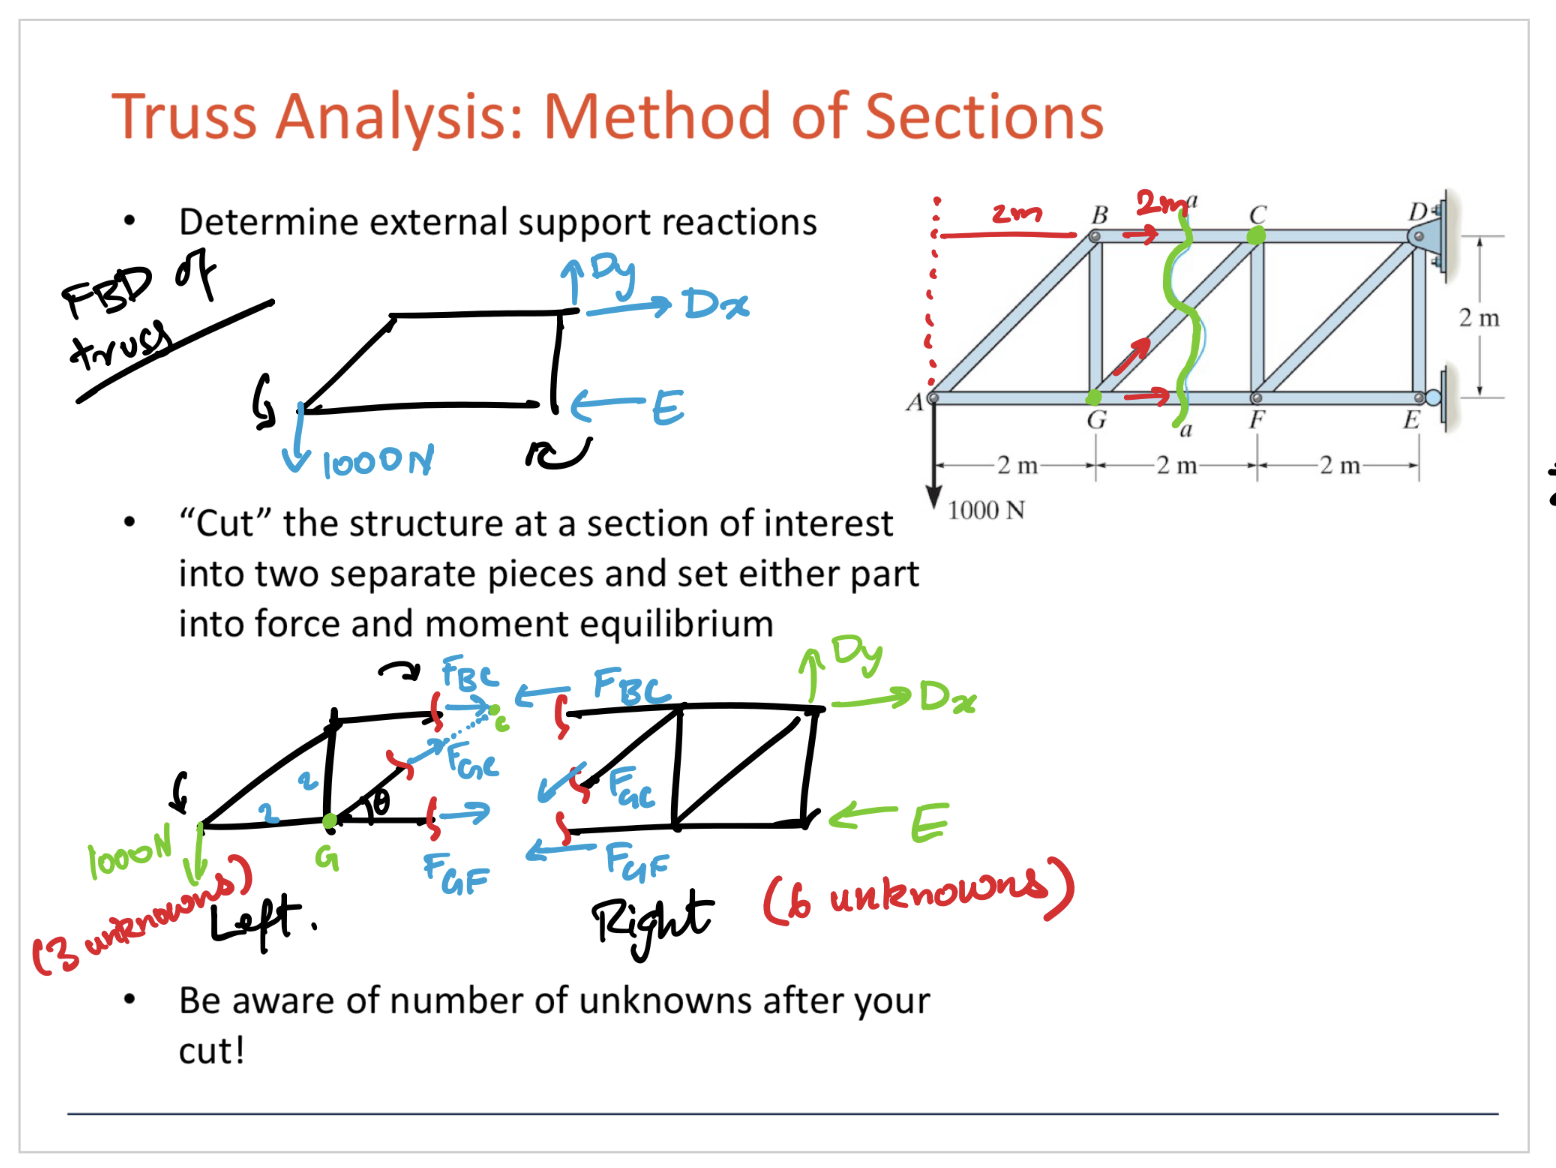
\includegraphics[angle=0, width=5in]{TrussFigures/MethodofSections.png}
\vspace{-2mm}
\caption{\small \blue{Taken from TAM 210 Lecture 19 notes}}
\vspace{-3mm}
\label{Fig:MethodofSections}
\end{figure*}

%lecture 19 



